\documentclass[10pt]{beamer}

\usetheme[progressbar=frametitle,sectionpage=none,subsectionpage=progressbar]{metropolis}
\setbeamertemplate{footline}{}
\usepackage{appendixnumberbeamer}

\usepackage{booktabs}
\usepackage[scale=2]{ccicons}

\usepackage{graphicx}
\usepackage{latexsym}
\usepackage{tikz}
\usetikzlibrary{patterns}  	%% for filling patterns
\usetikzlibrary{intersections}  %% 
\usetikzlibrary{shapes}  	%% e.g. allows nodes to have the shape of an ellipse
\usepackage{fp}  		%%% for arithmetics
\usetikzlibrary{calc, positioning}
\usetikzlibrary{matrix}
\usetikzlibrary{decorations}
\usetikzlibrary{decorations.text,decorations.markings,decorations.fractals,decorations.footprints,decorations.shapes}

\definecolor{mygray}{RGB}{200,200,200}
\definecolor{mygreen}{RGB}{64,114,122}
\definecolor{myorange}{RGB}{255,174,93}
\definecolor{myred}{RGB}{128,14,14}

\usepackage{pgfplots}
\pgfplotsset{compat=newest}
\usepgfplotslibrary{polar}

\usepackage[T1]{fontenc}
\usepackage{anyfontsize}
\usepackage{dsfont}

\usepackage{xspace}
\newcommand{\themename}{\textbf{\textsc{metropolis}}\xspace}

\usepackage{mathrsfs}
\usepackage{amsbsy}
% \usepackage{dsfont}
\usepackage[spanish, activeacute]{babel}
\usepackage[normalem]{ulem}
\usepackage[style=phys]{biblatex}
\bibliography{references}

\title{Profundidad de Datos Funcionales}
\date{Noviembre 2021}
\author{Nicolas Maldonado Baracaldo \newline 
Andrés Felipe Patiño López}
\institute{Departamento de Matemáticas\\Facultad de Ciencias\\Universidad de los Andes}
% \titlegraphic{\hfill\includegraphics[height=1.5cm]{logo.pdf}}

\begin{document}

\maketitle
{\fontfamily{cmr}
{\fontsize{10}{12}\selectfont


\section[Motivación]{Motivación}
\subsection{}

\begin{frame}{Motivación}

\invisible{m}

Para una muestra aleatoria real $X_1,X_2,...,X_n$ poemos definir:\pause
\begin{itemize}
    \item El $k$-ésimo estadístico de orden $X_{(k)}$.\pause
    \item El vector de rangos $\mathcal{R}=(R_1,\ldots,R_n)$. \pause
    \item $L$-estadísticos. En partícular, la media truncada. 
\end{itemize}

A lo largo de este curso, ya hemos visto la utilidad del vector de rangos y los estadísticos de orden.

% La media truncada, es decir, el promedio de los $n-[n\alpha]$ datos más cercanos a la mediana.  

\end{frame}

\begin{frame}{Motivación}
    \textbf{Profundidad:} Una medida de profundidad en un conjunto de datos proporciona una noción de centralidad de los mismos. Es una función $D:\mathbb{R}^k\to[0,1]$ que depende de la distribución de los datos (o de la empírica).\pause 
    \begin{itemize}
        \item Para finitos datos sin empates la profundidad induce estadísticos de orden.\pause
        \item La mediana será análoga al dato ``más profundo'' o ``más central''. Es decir, el estadístico de orden $X_{(1)}$. \pause
        \item Los datos atípicos o los datos extremos serán los ``menos profundos'' o ``menos centrales''. Por ejemplo, el estadístico de orden $X_{(n)}$. \pause
        \item Esto implica que las definiciones de profundidad son ligeramente diferentes en dimensiones $>1$.
    \end{itemize}
\end{frame}

\begin{frame}{Motivación}
    Debido a la naturaleza y la libertad de movimiento en dimensiones más altas, existen una gran variedad de formas de extender las profundidades de datos.
%Consecuentemente la definición de mediana. 
    Algunas profundidades (Datos multivariados): 
    \begin{itemize}
        \item \textbf{Tukey's Depth}
        \item \textbf{Simplicial Depth}
        \item \textbf{L1 Depth}
    \end{itemize}
\end{frame}

\begin{frame}{Motivación}
    
\end{frame}

\begin{frame}{Motivación}
    
\end{frame}

\begin{frame}{Motivación}
    \textbf{Objetivo:} Extender estas definiciones a $X_1(t),\cdots, X_n(t)$ datos funcionales i.i.d. $F_t$ con trayectorias continuas.\\[1cm]
\end{frame}

\section[Profundidad vía integración]{Profundidad vía integración}
\subsection{}

\begin{frame}{Profundidad vía integración}
    
    Suponga que tenemos una profundidad $D_t$ definida sobre $\mathbb{R}$ para cada $t\in [0,1]$ y $x(t)\in C[(0,1)]$. Defina:
    $$Z(t)=D_t(x(t)),\quad t\in [0,1]$$\pause
    La profundidad funcional (poblacional) de $x=x(t)$ es
    $$I(x)=\int_{0}^1Z(t)\;dt$$\pause
    \textbf{Obs:}
    \begin{itemize}
        \item Decimos que $x$ es profundo si $I(x)$ es grande.\pause
        \item Si los valores de $D_t(x(t))$ son pequeños (grandes), los valores de $I(x)$ serán pequeños (grandes).
    \end{itemize}
    %Es decir, si para muchos $t\in [0,1]$, $x(t)$ es profundo, I(x) será profundo. 
    
\end{frame}

\begin{frame}{EDO's and ranks}

    Dados $X_1(t),\ldots,X_n(t)$ procesos estocásticos i.i.d. con trayectorias continuas definidas en $[0,1]$, definimos 
    $$Z_i(t)=D_t(X_i(t))\quad\text{e}\quad I_i=\int_{0}^{1}Z_i(t)\;dt.$$
    
    Ordenamos los valores $I_k$ de forma decrecientes en profundidad. Si $I_j$ está en la posición $i$, entonces $X_{(i)}(t)=X_{j}(t)$. Esto es $R_j=i$ y $$X_{(R_j)}(t)=X_j(t).$$
    \textbf{Version muestral:} En la definición de la profundidad, reemplazamos $F_t$ por $F_{n,t}$ (la distribución empírica asociada) en la profundidad.
\end{frame}

\begin{frame}{Medias truncadas}
    Dado $\alpha>0$ (usualmente no superior 0.25). Podemos definir la media truncada a nivel $\alpha$ como el promedio de los $n-[n\alpha]$ datos más profundos.
    \\[1cm]
    Más precisamente, elegimos $\beta>0$ tal que el intervalo $[\beta, \infty)$ contenga $n-[n\alpha]$ valores de $I_n(X_i)$ para $i=1,\cdots, n$. Entonces:
    $$\widehat{\mu}_{n}=\frac{\sum_{i=1}^n\mathds{1}_{[\beta,\infty)}(I_n(X_i))X_i}{\sum_{i=1}^{n}\mathds{1}(I_n(X_i))}$$
\end{frame}

\begin{frame}{Consistencia}
    Bajo dos condiciones $H_1$ y $H_2$ uno puede garantizar que 
    $$\widehat{\mu}_n\to\mu\text{ c.s.}$$
    Donde 
    $$\mu=\frac{E(\mathds{1}_{[\beta,\infty)}(I(X_1))X_1)}{E(\mathds{1}_{[\beta,\infty)}(I(X_1)))}$$
    es la media poblacional recortada. 
\end{frame}

\section[Profundidad vía bandas]{Bandas}
\subsection{}

\begin{frame}{Profundidad vía bandas}
    El \textbf{grafo} de una curva $x\in C[a,b]$ está definido por:
    $$G(x)=\left\{(t,x(t)):t\in [a,b]\right\}$$
    Y, la \textbf{banda} delimitada por $j$ curvas $x_1,\ldots, x_j$ es:
    $$B(x_1,\ldots,x_j)=\left\{(t,y):t\in[a,b],\min_{k=1,\ldots,j}x_k(t)\leq y\leq \max_{k=1,\ldots,j}x_k(t) \right\}$$
\end{frame}

\begin{frame}{Profundidad vía bandas}
    \begin{figure}
        \centering
        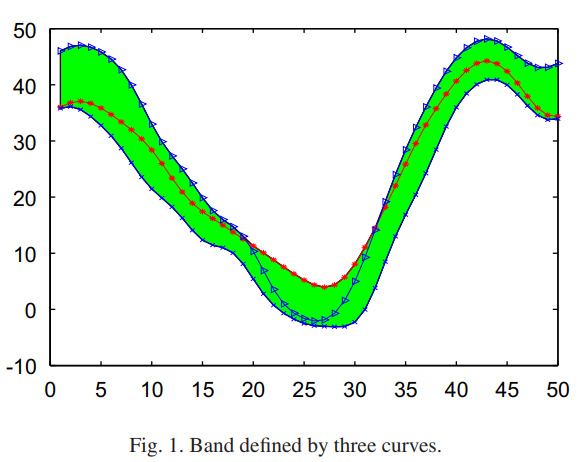
\includegraphics[width=7cm]{Picture2.png}
        %\caption{Caption}
        %\label{fig:my_label}
    \end{figure}
\end{frame}

\begin{frame}{BD}
    La medida de profundidad \textbf{BD} para una curva $x$ dado un conjunto de curvas $x_1,\cdots,x_n$ está dada por:
    $$S_{n,J}(x)=\sum_{j=2}^J S_n^{(j)}(x)$$
    donde 
    $$S_n^{(j)}(x)=\binom{n}{j}^{-1}\sum_{1\leq i_1\leq\cdots\leq i_j\leq n} \mathds{1}_{\{G(x)\subset B(x_{i_1},\cdots ,x_{i_j})\}}(x)$$
    % Esto generaliza la profundidad vía simplex o envolventes convexas. 
\end{frame}

\begin{frame}{BD}
\textbf{EDOs:}
Dados $X_1(t),\cdots,X_n(t)$ procesos estocásticos i.i.d.\pause
    \begin{itemize}
        \item La mediana se define como 
        $$X_{m}=\mathrm{argmax}\;S_{n,J}(X_i)$$
        \item \pause Puedo definir estadísticos de orden, rangos y medias truncadas con esta profundidad tal como antes.
    \end{itemize} 
\textbf{Restricciones:}\pause
\begin{itemize}
    \item Empates cuando $J=2$. \pause 
    \item Variabilidad y cálculo compuacional intensivo cuando $J>3$.
\end{itemize}
\end{frame}

\begin{frame}{BD}
    \begin{figure}
        \centering
        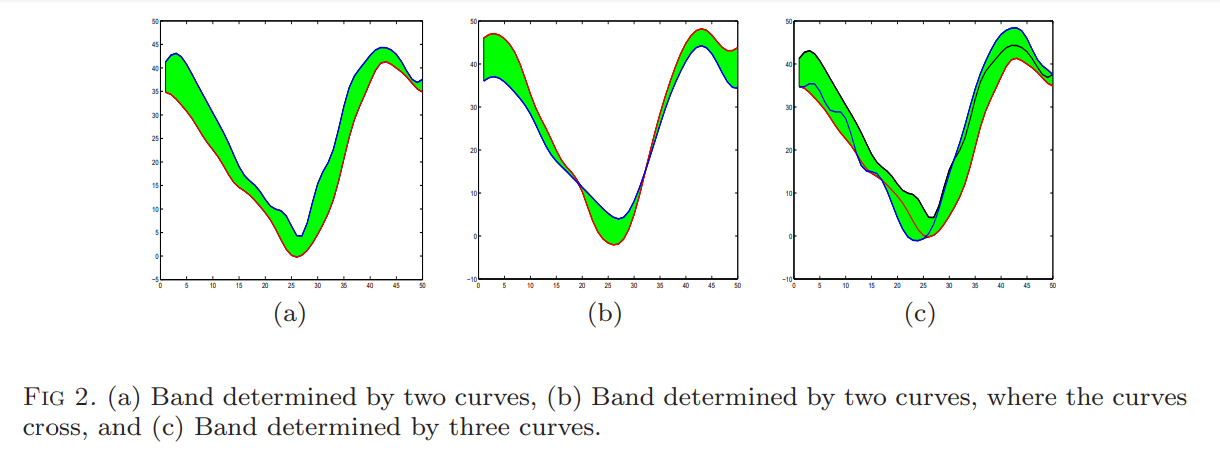
\includegraphics[width=10cm]{Picture3.png}
        %\caption{Caption}
        %\label{fig:my_label}
    \end{figure}
\end{frame}

\begin{frame}{BDG}
    \textbf{Idea:} Debilitar un poco la \textbf{BD} cambiando la función indicadora por la proporción de tiempo que una curva $x$ vive ``dentro'' de un conjunto de curvas dadas. 
    
    Considere las curvas $x,x_1,\ldots, x_n$ y para $j\leq n$ defina 
    $$A(x;x_{i_1},\ldots, x_{i_j})=\left\{t\in[a,b]:\min_{k=1,\ldots,j}x_{i_k}(t)\leq y\leq \max_{k=1,\ldots,j}x_{i_k}(t) \right\}$$
\end{frame}

\begin{frame}{BDG}
    Dados $x(t),x_1(t),\ldots,x_n(t)$ definimos la profundidad generalizada de banda \textbf{BGD} por
    $$GS_{n,J}(x)=\sum_{j=2}^{J}GS_{n}^{(j)}(x)$$    
    donde 
    $$GS_n^{(j)}(x):=\binom{n}{j}^{-1}\sum_{1\leq i_2\leq \cdots \leq i_j\leq n}\frac{A(x;x_{i_1},\cdots,x_{i_j})}{b-a}$$
\end{frame}

\section[Profundidad vía ``half-region'']{Bandas}
\subsection{}

\begin{frame}{Profundidad vía ``half-region''}
\textbf{Grafo, hipografo, epigrafo}
    \begin{align*}
        G(x)&=\left\{(t,x(t)):t\in[a,b]\right\}\\[0.4cm]
        hyp(x)&=\left\{(t,y)\in [a,b]\times \mathbb{R}:y\leq x(t)\right\}\\[0.4 cm]
        epi(x)&=\left\{(t,y)\in [a,b]\times \mathbb{R}:y\geq x(t)\right\}
    \end{align*}
\end{frame}

\begin{frame}{Profundidad vía ``half-region''}
    \begin{figure}
        \centering
        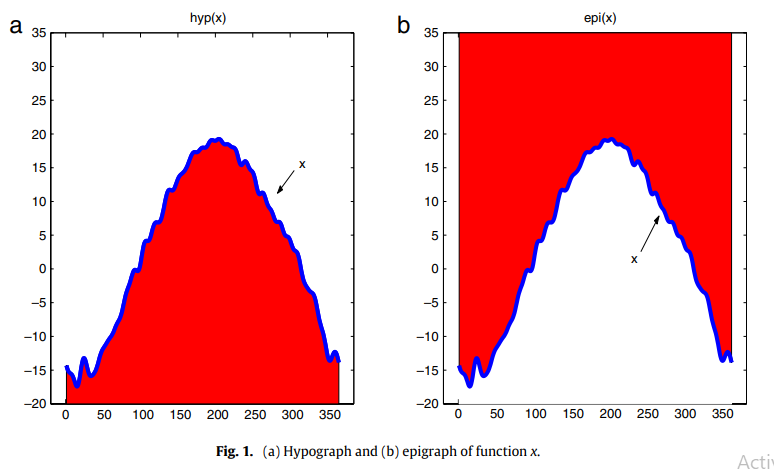
\includegraphics[width=9cm]{Picture1.png}
        %\caption{Caption}
        %\label{fig:my_label}
    \end{figure}
\end{frame}

\begin{frame}{Profundidad vía ``half-region''}
    Para una curva $x$ defina:
    \begin{align*}
      DG_1(x)&=P(G(x)\subset hyp(X))=P(x(t)\leq X(t),t\in [a,b])\\[0.2 cm]
      DG_2(x)&=P(G(x)\subset epi(S))=P(x(t)\geq X(t),t\in [a,b])
    \end{align*}
    Entonces la profundidad half-region (poblacional) de $x$ con respecto a $P$ es definida por:
    $$S_H(x)=\min\{DG_1(x),DG_2(x)\}$$
\end{frame}

\begin{frame}{Profundidad vía ``half-region''}
    La profundidad half-region de $x$ con respecto a $x_1,\ldots, x_n$ es:
    $$S_{n,H}(x)=\min\{DG_{1,n}(x),DG_{2,n}(x)\}$$
    donde 
    \begin{align*}
        DG_{1,n}(x)&=\frac{1}{n}\sum_{i=1}^{n}\mathds{1}_{\{G(x_i)\subset hyp(x)\}}(x)\\[0.2cm]
        DG_{2,n}(x)&=\frac{1}{n}\sum_{i=1}^{n}\mathds{1}_{\{G(x_i)\subset epi(x)\}}(x).
    \end{align*}
\end{frame}

\begin{frame}{Profundidad vía ``half-region''}
    Cómo en los ejemplos anteriores, podemos definir: mediana, estadísticos de orden, rangos y medias truncadas a nivel $\alpha$. 
    \begin{itemize}
        \item El dato que maximiza la profundidad es la mediana, es decir, 
        $$m_n=\mathrm{argmax}\;S_{n,H}(X)$$
        \item El dato que tiene la profundidad en la posición $k$-ésima es el estadístico de orden $X_{(k)}$ 
    \end{itemize}
\end{frame}

\begin{frame}{Profundidad vía ``half-region'' generalizada}
    De nuevo tenemos un problema similar con los empates. Por tanto, podemos debilitar la definición y considerar la proporción de  que la curva está en el epigrafo o en el hipografo. Es decir, para  
    \begin{align*}
        SL(x)&=\frac{1}{b-a}E[\lambda\left\{t\in[a,b]:x(t)\leq X(t)\right\}]\\
        IL(x)&=\frac{1}{b-a}E[\lambda\left\{t\in[a,b]:x(t)\geq X(t)\right\}]
    \end{align*}
    se define la profundidad:
    \[MS_H(x)=\min\{SL(x),IL(x)\}\]
\end{frame}

\begin{frame}{Profundidad vía ``half-region'' generalizada}
Con respecto a un conjunto de curvas $x_1,\ldots,x_n$ para
    \begin{align*}
        SL_n(x)&=\frac{1}{n(b-a)}\sum_{i=1}^{n}\lambda\{t\in[a,b]:x(t)\leq x_i(t)\}\\
        IL_n(x)&=\frac{1}{n(b-a)}\sum_{i=1}^{n}\lambda\{t\in[a,b]:x(t)\geq x_i(t)\}\\
    \end{align*}
    se define la profundidad
    $$MS_{n,H}(x)=\min\{SL_n(x),IL_n(x)\}$$
\end{frame}

\begin{frame}[standout]
    Gracias
    \rule[8pt]{\textwidth}{0.4pt}
\end{frame}

} %Fuente
} %Tamaño

\end{document}
